%!TEX TS-program = pdfLaTeX
%!TEX encoding = utf-8
%!TEX spellcheck = fr-FR

\documentclass[12pt,twoside,openright]{article}

%nœud

%\usepackage{soul}

%\documentclass[a4paper,11pt]{book}
\usepackage[T1]{fontenc}
\usepackage[utf8]{inputenc}
\usepackage[francais]{babel}

\usepackage[usenames,dvipsnames]{color}

\usepackage{lmodern}
%%%%%%%%%%%%%%%%%%%%%%%%%%%%%%%%%%%%%%%%%%%%%%%%%%%%%%%%%
% Source: http://en.wikibooks.org/wiki/LaTeX/Hyperlinks %
%%%%%%%%%%%%%%%%%%%%%%%%%%%%%%%%%%%%%%%%%%%%%%%%%%%%%%%%%
\usepackage{hyperref}
\usepackage{graphicx}
\usepackage{pdfpages}
\usepackage{amsmath}
\usepackage{amssymb}
\usepackage{a4}
\usepackage{indentfirst}
\usepackage{fancyhdr}
\usepackage{varioref}
\usepackage{makeidx}

%\usepackage{biblatex}
\usepackage{mslapa}

\usepackage[normalem]{ulem}



%% Apalike hyphenation %%%
%\let\oldbibitem=\bibitem
%\renewcommand{\bibitem}[2][]{\oldbibitem[#1]{#2}\newline}

%%% Margins %%%
\voffset -2.54cm
\textheight 24cm
\hoffset -1.3in
\evensidemargin 2.5cm
\oddsidemargin 2.5cm
\textwidth 18cm

% Book's title and subtitle
\title{\textbf{A three-party generative model for active foveated vision} }
% Author
\author{\textsc{Emmanuel Daucé}}%\thanks{\url{www.example.com}}}
\date{}
\makeindex

\begin{document}
	
\maketitle
	
	{\color{magenta} Notes :
	\begin{itemize}
		\item foveated vision models :  
		\item tree-structure representation of an image + saliency maps : used in image/video compression but not in computer vision
		\begin{itemize}
			\item Kortum + Geisler (1996) : foveated image encoding + multiresolution hierarchical encoding --> pyramid image encoding
			\item Serre + Poggio : multilayer encoding (+ haar wavelets(?))
			\item Francis Xinghang Chen = Poggio : pyramid encoding compression 
		\end{itemize} 	
		\item Neurosciences : 
		\begin{itemize}
			\item saliency maps + variants : Itti + Koch
		\end{itemize}
		\item MDP/POMDP/Bayesian models :
		\begin{itemize}
			\item Hinton, 2016 (!!) : http://papers.nips.cc/paper/6230-attend-infer-repeat-fast-scene-understanding-with-generative-models.pdf
			\item Friston (2017) : https://www.nature.com/articles/s41598-017-15249-0
			\item NIPS (2016) --> Markov blanket (pas POMDP) https://papers.nips.cc/paper/6039-sequential-neural-models-with-stochastic-layers.pdf
		\end{itemize}
		\item Connexion with IMOL : the most important part here...
		\begin{enumerate}
			\item estimation-based intrinsic reward
			\item connexion with extrinsic reward (last formula in IMOL abstract)
		\end{enumerate}
	\end{itemize}
	}
	
	
	The oculo-motor activity is an essential component of man and animal behavior, subserving most of daily displacements and interactions with objects, devices or people. By moving gaze with the eyes, the center of sight is constantly and actively moving around during all waking time.  %Though taking a large part in brain activity, the principles underlying those visually guided movements are still a subject of debate in neurosciences.
	Object recognition through saccades links to the case of a living system having to react at sort notice in a complex environment with limited sensors and limited computational resources. Under survival constraints and resource consuming optimization, not all the visual surroundings need to be scanned, but only the critical features, shapes and displacements. Few critical signals need to be interpreted fast, and many others can be ignored with no harm. This is the essence of visual orienting, a.k.a "active vision", that is present across most living species.  
	
	Understanding how robust and efficient visual orienting is achieved is important not only for neuroscience, but also for robotics, which faces similar constraints, in particular in the case of light and low-power sensing devices.  The active sensing framework primarily relies on emitting a signal to sense the environment, as is typically done by a radar or echolocation. Active vision (or active perception in general) generalizes to the concept of action-for-perception where a low resolution/low range sensing device is moved around to increase its range and/or its resolution, so that the computational and motor power may supplement the initial lack of sensing power. {\color{magenta} If the resulting device is significantly more complex, the global gain of sensing capabilities may be substantial.}
	  
	A similar problematic is emerging in various other fields, like e.g. machine learning, where the ever-growing  learning databases suggest to scan the data in a way that should retain only the critical examples and features to perform learning. Similarly, in computer vision, an active scan of high-resolution images may allow to overcome the limitations of current convolutional neural networks. Learning \emph{where to look at} seems to be an important field of investigation that may subserve large applicative outcomes.
	
	%is very popular in the field of robotics, and has gained significant revival in recent years through the development of   %both topics, both at the level of each objective  but also globally. %However, a property of the generic systems we propose is that they should 
	%As such, it is necessary to extend this problem to a generic set of conditions which are relevant to the trajectory of objects' contours in natural scenes, that is, for different configurations of the scene such as the presence of different types of objects.
	
	The concept of active vision and/or active perception is present in robotic literature under different acceptances. In \cite{aloimonos1988active}, the authors address the case of multi-view image processing of a scene, i.e. show that some ill-posed object recognition problems become well-posed problems as soon as several views on the  same object are considered. The term was also proposed in \cite{bajcsy1988active} as a roadmap for the development of artificial vision systems, that provides a first interpretation of active vision in the terms of sequential Bayesian estimation : \emph{{\color{blue} ``the problem  of Active Sensing can be stated as a problem of controlling strategies 
	applied to the data acquisition process which will depend on the current state 
	of the data interpretation and  the  goal  or the  task of  the  process.''}}.

	In physiology, the most documented case of active perception is gaze orienting, primarily studied in both man and animal \cite{yarbus1967eye,robinson1968eye}. Gaze orienting decomposes in several passive low-level reflex compensatory movements (vestibulo-ocular reflex, head stabilization, ...) as well as at least three active voluntary eye control modalities, i.e. visual anchoring, smooth pursuit and saccades that are at the core of vertebrate vision.  A nice review of principal promises of \emph{animate} vision against passive vision  is presented in \cite{ballard1991animate},  in relation with eye-hand coordination in computer vision.
	
	A saliant feature in superior vertebrates visual apparatus is the foveated retina that concentrates light photoreceptors over a small central portion of the visual field, {\color{magenta} following an approximate exponential decrease of resolution from the center to the periphery [REF?]}. The non-uniform distribution of photoreceptors across the retina provides both central high resolution and a wide field of view, but also imposes the animal to scan its visual surroundings to grab high spatial frequency information from different parts of the scene. This scan of the visual scene is principally done with high-speed targeted eye movements called saccades \cite{yarbus1967eye}, that sequentially capture local chunks of the visual scene. 
	
	The modelling of saccadic control offers thus an excellent testbed for addressing the more general active perception paradigm. It still presents many challenges, among which :
	\begin{itemize}
		\item efficiency
		\item oculomotor control and adaptation
		\item modelling and prediction
	\end{itemize}
	
	{\color{blue} Most importantly, for efficiency reasons, the scanning of the scene through saccades needs to be sparse, i.e. select the parts of the scene.
	Active vision needs to be encompassed in a full perception-action system view including the visual consequences of action, which emphasizes the importance of \emph{prediction} in visuomotor control \cite{Robinson1975,berthoz1996neural}} {\color{green} (attention Robinson propose un modele de prediction du mouvement lui-meme, pas des consequences visuelles du mouvement).}

    {\color{magenta} \uline{\bf NOTES BIBLIO  :}
    \begin{itemize}
    	\item {\bf Andrew Dankers, Alexander Zelinsky} --> Cedar (Hardware)
    	\item {\bf Ballard D (1991) Animate vision. Artif Intell 48:57–86} : stresses the importance of animate vision against passive vision. 
    	\begin{itemize}
    		\item \emph{``At any rate, having a particular embodiment forces
    			one to deal with performance issues: One has to act in a timely manner under resource constraints.
    			One way to do this would be to have an elaborate internal representation as a form or "table lookup." But in a dynamic world, the cost of maintaining the correspondence between the representation and the world becomes prohibitive. For this reason animate vision systems \uline{may have to travel light} and depend on highly adaptive behaviors that can quickly discover how to use current context.''}
    		\item \emph{`` Gaze control mechanisms fundamentally change computational models of vision. Without
    			them the visual system must work in isolation, with the burden of solving difficult problems with
    			many degrees of freedom. With them a new paradigm emerges in which the visual calculations are
    			embedded in a sensory-motor behavioral repertoire. Rather than thinking of visual
    			processing as separate from cognitive or motor processing, they are interlinked
    			in terms of integral behaviors''}
    		\item independant controllers operating in parallel	(Yamauchi 1989)
    		\item \emph{``A gross distinction that
    			can be made is between identification algorithms that analyze the foveated area during fixation and
    			location algorithms that direct the eyes to new targets. Support for this WHAT/WHERE distinction, made by Mishkin [Mishkin 1982; Mishkin et al. 1983].''}
    	\end{itemize}
    	\item  {\bf Brooks A, Abdallah S, Zelinsky A, Kieffer J (1998)} A mul-
    	timodal approach to real-time active vision. In: International
    	conference on intelligent robotics --> chez Brooks, l'orientation du regard est en lien avec l'interaction et la communication homme/machine.
    	\item {\bf Dickmanns ED (1999) An exception-based, multi-focal, sac-
    		cadic (ems) vision system for vehicle guidance. In: Proc. inter-
    		national symposium on robotics and research}
    	\item Computer vision
    	\item Event-based coding and event-based  sensors?
    	\item Foveated vision (and models)
    \end{itemize}	}
    
    
	{\color{green} Idee de simuler les conséquences de l'action (voir le chapitre de Berthoz dans le bouquin de Damasio) --> "perception is a decision"}

	{\color{green} La vision active pour le computer vision ne s'est pas tellement développée du fait du coût decroissant du traitement d'images et de la facilité à paralléliser les traitements.}
	
	\section{Model}
	
	\subsection{probabilistic modelling}

	The active vision paradigm was recently introduced in neuroscience through the work of ~\cite{friston2010free,friston2012perceptions}. % 
	The general setup proposed by Friston and colleagues is that of a general tendency of the brain to counteract surprising and unpredictible sensory events through building generative models that improve their predictions over time and render the world more amenable. This improvement is mainly done through sampling the environment and extracting statistical invariants that are used in return to predict upcoming events.
	Building a model thus rests on extracting a repertoire of invariants and organizing them so as to process the incoming sensory data efficiently through predictive coding \cite{rao1999predictive}. This proposition, gathered under the ``Variational Free Energy Minimization'' umbrella, has important consequences for it formally links two important domains of investigation, namely dictionary construction from data through machine learning and (optimal) motor control.
	In particular, motor control is here considered as a particular implementation of a \emph{sampling process}, that is at the core of the estimation of a complex posterior distribution. 
	
	The active inference approach relies on a longstanding history of probabilistic modelling in signal processing and control \cite{Kalman1960,Baum1966,friston1994statistical}.  Put formally, the physical world  takes the form of a generative process $p$ that is the cause of the sensory stream. This process is not visible in itself but is only sensed through a (non reliable) measure process that provides an observation vector $x$. The inference problem consists in estimating the underlying causes of the observation, that rests on a latent state vector $z$ and a control $u$.  Then, the evolution of $x$ relies on both $u$ and $z$ in the form of a stochastic dynamical system undergoing an external forcing command $u$, i.e. :
	\begin{align}
	  \dot{z} &= A(z) + B(u) + \text{process noise}\label{eq:kalman-process}\\
	  x &= C(z) + D(u) + \text{measurement noise} \label{eq:kalman-measure}
	\end{align}  
	where $A$, $B$, $C$ and $D$ constitute a generative model $p(x,u,(z,\dot{z}))$ that explicits the dependencies between $u$, $x$ and $z$ \footnote{We note for simplicity $p(x,u,z)$ in the following, with each variable counting for its state vector and possible higher moments.}. 
	The calculation of $z$ from $u$ and $x$ relies on $p = \{A,B,C,D,\text{noise models}\}$. The model can then be inverted in order to compensate the drift of the state estimate \cite{Kalman1960,Baum1966}. The more accurate the model, the better this estimation. 
	
	\subsection{Perception-driven control}
	The question we address here is the design a \emph{controller} $C$ that outputs a control $u$ so as to maximize the accuracy of this state estimation process. This is the purpose of a \emph{perception-driven} controller.
	{\color{magenta} In the following, $z$ is the \emph{scene encoding}, corresponding to the positions of sensible objects surrounding the controller, independently of the sensor orientation}, by opposition to $x$ which is the ``sensory patch'' or ``sensory field'' provided by the sensors. {\color{blue} The sensory field relies on the orientation of a mobile device that is controllable through a certain number of degrees of freedom (pan, tilt and roll for a visual sensor for instance). A control $u$ is then a vector that affects those different degrees of freedom through an actuator.} The knowledge about $z$ (scene encoding) then relies on the sensory patches $x$'s that are collected through changing $u$ (sensor orientation) across time. 
	
	Now, the general objective of an \emph{active inference} framework is to choose $u$ appropriately in order to minimize the uncertainty about the cause of the perception, i.e. to identify the scene components $z$. 
	This knowledge about the sensory scene can be reflected in a distribution $q(z)$. The better the knowledge (precision) about a sensory scene, the lower the \emph{entropy} of $q$, with:
	$$H(q) = E_z[- \log q(z)]$$
	It is shown in \cite{friston2012perceptions} that minimizing the entropy (or maximizing the ``salience'') through action can be linked to minimizing the variational free energy attached to the future observation $x$ (see appendix{\ref{appendix-friston}).
		
		
	
	At each step of the sensing process, the distribution of $q$ is updated according to the new observations. The control $u$ is expected to be optimal, i.e. to reduce at most the entropy of $q(z)$ at each step. This optimal $u$ is not known in advance, because $x$ is only read \emph{after} $u$ has been carried out. Then comes the predictive framework that identifies the effect of $u$ with its most probable outcome, according to the predictive model.
	
	In our feedback control framework, given a generative model $p$, and an initial condition $z_0$ (or initial guess), a control $u \in \mathcal{U}$ allows to make a \emph{prediction} about a forthcoming $z$, which allows in turn to make a prediction about the forthcoming $x$. Those predictions take the form of two conditional distributions, namely $p(z|u,z_0)$ and $p(x|z,u)$ according to (\ref{eq:kalman-process} and (\ref{eq:kalman-measure})). %, which allows to predict the next $p(x,z|u,z_0) = p(x|z,u) p(z|u,z_0) = p(z|x,u,z_0)p(x|u,z_0)$.
	Then, the forthcoming posterior distribution is (Bayes rule):
	\begin{align*}
	p(z|x,u,z_0) &= \frac{p(x,z|u,z_0)}{p(x|u,z_0)}\\
	             &= \frac{p(x|z,u) p(z|u,z_0)}{\sum_{z'}p(x|z',u) p(z'|u,z_0)}
	\end{align*}
	so that the forthcoming entropy is:
	\begin{align*}
	H(q)|_{u, z_0} &=  E_{x,z}\left[-\log  p(z|x,u,z_0)\right]
	\end{align*}
	and the optimal $u$ is:
	\begin{align*}
	\hat{u} &= \underset{u \in \mathcal{U}}{\text{argmin }} H(q)|_{u, z_0} \\
	\end{align*}
	with:
	\begin{align*}
		q(z)|_{u,z_0} &= p(z|x,u,z_0) \\
	\end{align*}
	
	In practice, the analytic formulations are generally out of reach (in particular for predicting the next sensory field $x$).  One thus need to consider an \emph{estimate} $\tilde{u} \simeq \hat{u}$ that should rely on sampling from the generative process $p$ to 
			predict the effect of $u$,  i.e. 
			$$ \tilde{u} = \underset{u}{\text{argmin}} \frac{1}{N} \sum_{i = 1..N, x_i \sim p, z_i \in \mathcal{Z}} -\log p(z_i| x_i, u, z_0) $$ or on an even sharper direct estimation through maximum likelihood estimates (point estimate):
			\begin{align*}
				&\tilde{u} = \underset{u}{\text{argmin }} - \log p(z_\text{max}|x_\text{max}, u, z_0)	\\
				&z_\text{max} = \underset{z}{\text{argmax }} p(z|x_\text{max}, u, z_0)\\
				&x_\text{max} = \underset{x}{\text{argmax }} p(x|u,z_0)
			\end{align*}
		}
	
	This operation can be repeated in a sequence, where the actual control $u = \tilde{u}$ is followed by reading the actual visual field $x$, which in turn allows to update the actual posterior distribution over $z$. This updated posterior becomes the prior of the next decision step, i.e. $z_0'\sim  p(z|x, u, z_0)$ so that a new control $u'$ can be carried out etc. 
	
	If we denote $T$ the final step of the process,  with $u_{1:T}$ the actual sequence of controls and $x_{1:T}$ the actual sequence of observations, the final posterior estimate becomes $p(z_{1:T}|z_0, u_{1:T}, x_{1:T})$.
	
	%{\color{blue} Put in a sequential setup :
	%	\begin{align*}
	%	&\tilde{u}_{1:T} = \underset{u_{1:T}}{\text{argmin }} - \log p(z^\text{max}_{1:T}|x^\text{max}_{1:T}, u_{1:T}, z_0)	\\
	%	&z^\text{max}_{1:T} = \underset{z_{1:T}}{\text{argmax }} p(z_{1:T}|x^\text{max}_{1:T}, u_{1:T}, z_0)\\
	%	&x^\text{max}_{1:T} = \underset{x_{1:T}}{\text{argmax }} p(x_{1:T}|u_{1:T},z_0)
	%	\end{align*}
	%	}
 

	
	
		{\color{green} From this general standpoint, many familiar methods and principles naturally derive when considering additional details or simplifying assumptions... MODEL-BASED, SAMPLING, LEARNING (post-hoc optimization), ...}
		
		{\color{green} from sampling $x$ from the generative process through $u$, which entail well-described form of exploration-exploitation optimization learning process [REF].}
		
		
	
	
	
	\subsection{Visuo-motor control}
	
	encoding distribution $q$
	
	decoding distribution : $p$
	
	visual orientation : $u$
	
	visual field : $x$
	
	\emph{steady state assumption}, i.e. $\dot{z} = 0$
	
	We considers an organization a the visual scene in objects (or causes), whose presence and position is continuously checked by visual inspection. Here saccades are considered to probe a particular region of the visual scene, with the objective of reducing the uncertainty about the identity and position of particular objects. %This theory takes for granted that an a priori knowledge exists on all possible objects and locations but also for the repertoire of movements.
	 	
	 Put formally, exploring a visual scene through saccades consists in identifying objects in space through the foveation of parts of the scene only. The cause of the current visual field $x$ is both the object identity $o$, its position in the peripersonal space $y$, and the current visual orientation $u$, i.e. $x \sim P(X|y,o,u)$, each variable counting for a distinct degree of freedom. % and the generative process  for every possible composition of object identity $o \in \mathcal{O}$, position $x \in \mathcal{X}$ and $u \in \mathcal{U}$. 
	 In a model-based approach, with $P$ the generative process, the active vision paradigm mainly considers optimizing the choice of $u$ for reducing uncertainty about $y$ and $o$, which are the undisclosed constituents of the scene. For simplicity $y$ and $o$ are here reduced to a single variable $z = (y, o)$. Considering now that a certain prior $\pi(z)$ has been formed about $z$, choosing  $u$ conducts the sight in a region of the visual field that provides $y$, which in turn allows to refine the expectations about the cause of the perception, i.e.
	 $ P(z|u,y) \propto P(y|z,u) \pi(z)$. 
	 One needs thus to choose $u$ appropriately in order to reduce the uncertainty about $z$, given the actual $y$, i.e minimize the entropy :
	 $u^* = \underset{u \in \mathcal{U}}{\text{argmin }} H$ with $H = E(-\log P(z|u,y))$.
	 
	 
	 In that framework, saccadic exploration means thus to define a sequence of visuo-motor commands $\tilde{u}$, $\tilde{u}'$, $\tilde{u}''$, ... This sequence should ultimately provide a final estimate $\pi^{(n)}(z)$ such that a single cause $\hat{z}$ may dominate the other ones, allowing the system to reach a final decision.  
	 
	 {\color{blue}
	 	This can for instance be done under a greedy setup, i.e. first set $\tilde{z} = \underset{z \in \mathcal{Z}}{\text{argmax }} \pi(z)$, second set $\forall u, \tilde{y}_u = \underset{y \in \mathcal{Y}}{\text{argmax }} P(y|\tilde{z},u)$.
	 	Finally, set 
	 	\begin{equation}
	 	\tilde{u} = \underset{u \in \mathcal{U}}{\text{argmax }}  P(\tilde{z}|u,\tilde{y}_u))
	 	\end{equation} which is a proxy for minimizing the entropy. This greedy choice tells in short that if $\tilde{z}$ is the running hypothesis, the operator should orientate his sight toward 
	 	%the part of the scene where he thinks his assumption should receive confirmation, i.e. 
	 	the part of the scene that is the most discriminative toward confirming $\tilde{z}$ against all other possibilities. }
	 
	 \section*{Notes}
	
	%Instead, $u$ should be sampled from a an estimation of $L = - \log p(x, z, u')$ needs to be defined to approximate one should consider sampling the 
	
	{\color{blue}
	LEARNING (ici on sépare le modèleinterne (estimation) du modèle externe ==> model free, encodage...) The variational distribution $q$ (the approximate posterior) also provides a way to refine the estimation of $p$. From the classical image processing and machine learning standpoint, $q(z|x)$ is called the \emph{encoder} that maps a feature vector $x$ toward its redescription $z \in \mathcal{Z}$ (in the latent variable space). In control theory, $q$ is an inverse model that maps the input $x$ toward its hidden cause $z$ etc. Conversely, $p(x,z)$ (the generative distribution) is a \emph{decoder} that generates samples from their causes (namely carries out the visual consequence of a certain emitter $z$), or a \emph{forward model} in the terms of control theory.}
	
	{\color{blue} (ORIGINAL? Voir COMMENT CA SE DEMARQUE DE FRISTON?) 
		
	Friston/Perrinet : \emph{``The brain minimizes the free energy of sensory inputs defined by a generative model. This model includes prior expectations about hidden controls that maximize salience.	 
	The prior beliefs considered below pertain to these hidden controls and dictate how we engage actively with the environment to minimize the uncertainty of our perceptual inferences. Crucially, this means that prior beliefs have to be encoded physically (neuronally) leading to the notion of fictive or counterfactual representations; in other words, what we would infer about the world, if we sample it in a particularly way. This leads naturally to the internal representation of prior beliefs about fictive sampling and the emergence of things like intention and salience.''} --> c'est l'idée de simulation (semble-t-il) des consequences de l'action avec le modele generatif. La lien avec l'intention et la saillance n'est pas clair (a moins qu'il s'agisse d'extraire les caracteristiques saillantes de l'objet suposé). En ce qui concerne le prior, il s'agitrait simplement d'un modele generatif sur (z,u). il faut voir dans quelle mesure l'hypothèse de "steady state" est exploitée)
		
	In order to XXX, we propose to split the generative process in two parts, namely the controlled generative process and the uncontrolled generative process. The controlled emitter is named $u$ while the uncontrolled emitter is named $z$. The value of $u$ refers to the state of a motor apparatus, e.g. to the spatial distribution of the different mobile segments of an articulated body. The value of $z$ refers to the remaining part of the physical world, i.e. the "environment". This restricted setup, that separates a body and an environment the form of two parallel processes,  provides a substantial simplification to the estimation problem at stake.  	
	
	An additional assumption is that the controlled generative process is relatively "fast" in comparison with the uncontrolled one. In consequence we reduce $u$ to  a motor setpoint (a motor command) that is supposed to be realized by the motor apparatus at short notice under classical stability/controllability constraints.
	

	
	Then the latent state space (the cause of the visual field) decomposes in a hidden cause $z$ and an explicit motor control $u$. The generative distribution becomes $p(x, z, u)$ so that activating the motor effectors updates the state of the plant as well as its visual sensory outcome. In comparison,  changing the state of an external (uncontrolled) emitter would also modify the visual sensory outcome. The command $u$ here participates in a feedback loop that in return updates the visual stream.
		
	In the particular case where $u$ and $z$ can be set independently, a prior $\pi(z)$ can be set on $z$ so that $q(z,u|x)$ rewrites $q(u|z,x)\pi(z)$ and $p(x, z, u)$ rewrites $p(x, u |z) \pi(z)$. In that particular setup, the hidden cause $z$ plays the role of a generative model on $x$ and $u$. The free energy minimization assumption tells that $u$ should minimize the surprise caused by the future observation $x$, where $x$ is the actualization of the generative process $p$ given the control $u$. 
	If $p$ is known (model-based case), then the optimal control is
	$$u^* = \underset{u}{\text{argmin}} \int \int - \log p(x|z, u) \pi(z) dx dz$$
	which is generally intractable on large-dimension input state spaces.
	
	An approximate optimal control can be obtained through sampling $u$ (and $z$) and estimating its future visual consequences.
	
	When $p$ is known in approximation only (with $\tilde{p}$ an estimate of $p$)
		$$u^* = $$ A non-biased estimator of $F$ can then be obtained through the sampling }
		

	
	(for instance a needle in a haystack, or a puzzle),  and a set of several possible hidden causes, action consists in manipulating the environment so as to remove ambiguities and provide a clearer view of the setup. 
	
	{\color{blue} le sampling repose sur un processus d'estimation d'une distribution difficile à calculer. En lien avec l'idée de variable auxilliaire. Le fait de sampler une cause (l'aiguille est en (x,y)) conduit à produire la direction de regard (x,y). Autrement dit $u$ est une hypothèse du modèle génératif. }
	
	
	
	{\color{blue}
		
		
		An additional intuition that comes out from
		
		To do so, they recast the traditional perception-action control loop in  		 
	
		
		
		Friston and colleagues postulate that the brain is a controller that acts on its environment 
		
		The general concepts manipulated by the Free Energy framework are the maintenance of a physical system in a relatively low entropy state through counteracting a general tendency to disorder. 
		
		Put in a visuomotor control context, 
		
	}
	
	
	
	{\color{magenta} Sequential Bayesian estimation with stopping criterion} 
	
	For illustrative purpose, this setup was tested on a classic machine learning image processing setup, namely the MNIST dataset. In order to mimic a foveated exploration, a 2D-wavelet decomposition is performed on the images, providing a series of triplets of wavelet coefficients organized in space and in different levels. A visual orientation command $u = (i,j)$ then allows to read out several wavelets coefficient triplets associated with the considered coordinate (at different levels). Given a model $P(y|u,z)$, each  wavelet coefficients triplet $y$ is thus expected to participate in uncovering the underlying object $z$ (here a digit between 0 and 9).

	\begin{figure}[t!]
		\centerline{
				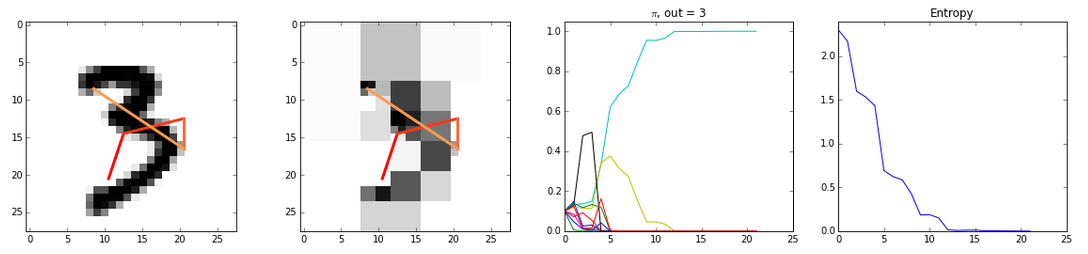
\includegraphics[width = \linewidth]{img/figure.png} 
		}
		\centerline{\bf a \hspace{4cm} b \hspace{4cm} c \hspace{4cm} d}
		\caption{\footnotesize{{\bf Saccadic exploration for digit image recognition}~. {\bf a.} Saccades trajectory (from red to orange) superimposed over an original digit. {\bf b.} Saccades trajectory over reconstructed image from available visual information. {\bf c.} Posterior probability update, in function of the number of wavelet triplets observed. {\bf d.} Entropy of the posterior, in function of the number of wavelet triplets observed. } }
	\end{figure}
	
	The predictive model is built on a 55,000 exampleFrom this general standpoint, many familiar methods and principles naturally derive when considering additional details or simplifying assumptions... MODEL-BASED, SAMPLING, LEARNING (post-hoc optimization), ...
	
	{\color{blue} from sampling $x$ from the generative process through $u$, which entail well-described form of exploration-exploitation optimization learning process [REF].}
	
	{\color{magenta} Instead, one need to consider an estimate $\tilde{u}$ that should rely on sampling from the generative processes $p$ and $q$ to 
		predict the effect of $u$,  i.e. 
		$$ \tilde{u} = \underset{u'}{\text{argmin}} - \frac{1}{N} \sum_{\{z_i, x_i\}_{i = 1..N, z \sim q, x \sim p}} \log p(x_i, z_i, u') $$ or on direct estimation through maximum likelihood estimates (point estimate):
		\begin{align*}
		&z_\text{max} = \underset{z}{\text{argmax }}q(z)\\
		&x_\text{max} = \underset{x}{\text{argmax }} p(x|z,u')\\
		&\hat{u} = \underset{u'}{\text{argmin }} - \log p(x_\text{max}, z_\text{max}, u')
		\end{align*}
	} set, and reaches approximately 92 \% correct recognition on the test set. The image decomposition in a dictionary of wavelets coefficients is rather rough, though providing a simple validation of the proposed setup. The performance is also quite satisfying given the model lightness, when compared to tedious layered dictionary construction in convolutional neural networks. 
	More importantly, the decision over the predicted posterior (eq. 1), that scans all possible outcomes of actions, can be pre-processed and stored in a table to simplify decision. The structure of the decision process is moreover consistent with the reinforcement and online learning frameworks, with action outcome possibly assimilated with the (log)-likelihood of the visual field, and/or with higher level target reaching/achievement criterions.
	
	{\color{magenta} The artificial curiosity framework posits that the part of the visual scene being the less congruent with the current assumption should attract visual attention. Choosing the part of the scene with the highest discriminative power maximises the chance to find the visual input sur
		
		where the chance to find a non-congruent visual input is the highest, i.e.
		$$ \underset{u}{\text{argmin }} P(y|z,u) P(z)$$
		This idea 
		Regarding the artificial curiosity thematic, the model presented her posits that the model is attracted by regions of the visual field that should maximize the surprise if the current assumption is wrong}
	
	{\color{magenta} Our hypothesis is that efficient object-specific saccade sequences may be pre-learned to facilitate recognition under prior assumptions about the state of the environment. }
		
		
	
	
	%
	
	%Taking guidance from the biological observations, the idea is to consider the natural strategies adopted to deal with limited sensors and limited computing resources.
	%: how use at best low sensory bitrate and noisy sensors? how much memory use, what motor decisions make to maintain a consistent model of the outside scene? 
\begin{footnotesize}
\bibliographystyle{apalike}
\bibliography{biblio}
\end{footnotesize}	
	
\appendix
\section{Appendix}\label{appendix-friston}
{\color{magenta} The funding assumption of the active inference framework is that the choice of $u$ (i.e the control law) should rest on minimizing the entropy of the sensory field, i.e. minimizing the surprise caused by a new visual input $x$ knowing that $z$ is under the control of $u$. This quantity, called the ``surprise'', is the negative log evidence of the data stream, i.e $-\log p(x)$ (the marginal over $z$ and $u$), so that choosing $u$ means to optimize $-\log p(x|u)$:
	
	$$ \hat{u} = \underset{u \in \mathcal{U}}{\text{argmin}} \langle -\log p(x|u)\rangle_{z\sim p}$$
	
	This assumption of surprise minimization needs to be done under certain known conditions (the priors) about the generative process $p$. Those priors need to be set at some point, otherwise active inference should reduce to orienting the sensors toward region of the sensory scene that is the easiest to predict  (for instance orientate sight toward the darkest  part of the scene (dark room problem) [REF]). 
	
	%{\color{green}
	%For instance, let us consider $z$ be a "real" state of the world ("perfect" prior). Then the optimal choice of $u$ should rest on maximizing the accuracy of predicting $x$ given $u$ and $z$, i.e. 
	%$$ \hat{u \in \mathcal{U}} = \underset{u}{\text{argmax}} \log p(x|z,u)$$
	%}
	
	Setting a prior over the generative process rests on the design of a ``variational'' distribution $q$ that puts a bias on the generative process according to either an a priori knowledge or on parts of the world that are actually known or sensed.
	$$ \hat{u} = \underset{u \in \mathcal{U}}{\text{argmin}} \langle -\log p(x|u)\rangle_{z\sim q}$$ 
	Then the reduction of surprise can rest on optimizing $q$ with respect to $u$ (instead of $p$).  In practice, the surprise caused by $x$ will be minimized if the \emph{entropy} of $q$ is minimized \cite{friston2012perceptions}, i.e.:
	$$ \hat{u} = \underset{u \in \mathcal{U}}{\text{argmin}} \langle -\log q(z)\rangle_{z \sim q\text{, }x\sim p(.|z,u)}$$ 
	with $x$ corresponding to one sample observation and $q$ approaching the ``real'' posterior with its estimate $p(.|x,u)$, so that finally:
	$$\hat{u} = \underset{u \in \mathcal{U}}{\text{argmin }} H$$ 
	with:
	$$H = E_z(-\log p(z|x,u))$$
}
%Put in the terms of a control law, the choice of $u$ relies on optimizing $u$ with respect to the objective $F$, i.e. finding the $x$ that is maximally consistent with $z$ given $u$ :
%$$ u = \underset{u'}{\text{argmin }} \langle - \log p(x, z, u')\rangle_{z\sim q}$$ 
%which is generally not tractable. Instead a control policy $u \sim \pi(z)$ needs to be set, that approximates the previous expression, depending on the control setup at stake.    



\end{document}